\chapter{Background}

This chapter presents knowledge graphs and different paradigms for how to interpret information missing from a \gls{kg}. Then we continue with knowledge graph embeddings where we examine the training and evaluation process and explain the ideas behind the three knowledge graph embedding architectures used in the experiments. Finally, the chapter introduces rule mining by first giving a general overview of rule-based machine learning before focusing on the \textit{association rule mining} approach.

\section{Knowledge Graphs}
There is no single agreed-upon definition of \glspl{kg} \cite{bergman_2019, bonatti2019knowledge, ehrlinger2016towards}. Definitions and usages vary from specific technical proposals to more general descriptions. In this thesis, we use the more inclusive definition similar to the one proposed by Hogan et al. \cite{hogan2020knowledge}, where we view a \gls{kg} as \textit{a graph of data intended to capture the semantic connections within real world knowledge, where nodes represent relevant entities and edges represent relations between these entities}. The type of graph may vary, i.e. it may be simple, directed, etc. A graph may contain knowledge over a broad range of domains, such as Wikidata~\cite{lehmann2015dbpedia}, or be limited to a specific domain, such as DBpedia \cite{fellbaum2010wordnet}. The concept of ``knowledge'' has been widely debated in epistemology \cite{chappell2005plato, kirkham1984does, wittgenstein1969certainty, gottschalk2008internet}, but here we use it to mean descriptive knowledge, meaning facts that can be stated. Knowledge can be simple statements, such as ``\textit{Leo is a cat}'', or quantified statements such as ``\textit{at least one cat is black}''. %\glspl{kg} are not expressive enough for quantified statements, where ontologies or rules would be more appropriate. 
Additional knowledge can be inferred from \glspl{kg} through inductive or deductive methods. For example from a \gls{kg} containing the information that ``\textit{Leo is a cat}'' and ``\textit{cats are mammals}'', one can deductively infer that ``\textit{Leo is a mammal}''. If all cats mentioned in the knowledge graph like to eat fish, then one can inductively infer ``\textit{cats like to eat fish}''.

\begin{figure}[htbp]
\centering
\begin{tikzpicture}
    \node[shape=circle,draw=black] (L) at (0,0) {Leo};
    \node[shape=circle,draw=black] (C) at (3,0) {Cat};
    \node[shape=circle,draw=black] (M) at (1.5,3) {Mammal};

   % \path [->] (L) edge node[left] {$IsA$} (C);
   \draw [->] (L) -- (C);
   \draw [decoration={text along path,
    text={is a},text align={center}},decorate]  (L) -- (C);
    
    \draw [->] (C) -- (M);
   \draw [decoration={text along path,
    text={subclass},text align={center}},decorate]  (M) -- (C);
    
    \draw [dotted, ->] (L) -- (M);
   \draw [decoration={text along path,
    text={is a},text align={center}},decorate]  (L) -- (M);
    
\end{tikzpicture}

\caption[Simple visual example of a KG.]{Example of a \gls{kg}, where the dotted line represents a relationship that can be deductively inferred.} \label{fig:KGexample}
\end{figure}

In this thesis we loosely follow the \gls{rdf} standard and view \glspl{kg} as sets of semantic triples. \gls{rdf} is a standard for representation and exchange of graph data introduced by \gls{w3c}. Semantic triples are the data types used in the \gls{rdf} data model. A triple, as the name suggests, is a tuple of three elements. It has the form (subject, predicate, object) and can therefore represent statements about semantic data, for example ``\textit{cats are mammals}", or ``\textit{Ann knows Bob}". 
\begin{lstlisting}[caption={Example of RDF triple set written in informal pseudocode.}, label={RDF_triples_example}]
(Leo, is_a, cat)
(cat, is_a, mammal)
(Ann, is_a, person)
(Bob, is_a, person)
(Ann, knows, Bob)
(Ann, has_pet, Leo)
\end{lstlisting}
\gls{rdf} statements express relationships between two web resources, these resources being the subject and the object, while the predicate encapsulates the nature of the relationship. The relationship is phrased in a directional way, and so a set of \gls{rdf} statements can also be viewed as a directed graph. The graph represents these triple statements, where the predicate in the triple denotes the edge going from the subject to the object, both of which are vertices.

\begin{figure}[htbp]
\centering
\begin{tikzpicture}
    \node[shape=circle,draw=black] (L) at (3.9,0) {Leo};
    \node[shape=circle,draw=black] (P) at (0,2.5) {Person};
    \node[shape=circle,draw=black] (A) at (1,0) {Ann};
    \node[shape=circle,draw=black] (B) at (2.5,2.5) {Bob};
    \node[shape=circle,draw=black] (C) at (6,0) {Cat};
    \node[shape=circle,draw=black] (M) at (5,2.5) {Mammal};

   % \path [->] (L) edge node[left] {$IsA$} (C);
   \draw [->] (L) -- (C);
   \draw [decoration={text along path,
    text={is a},text align={center}},decorate]  (L) -- (C);
    
    \draw [->] (L) -- (M);
   \draw [decoration={text along path,
    text={is a},text align={center}},decorate]  (L) -- (M);
    
    \draw [->] (A) -- (B);
   \draw [decoration={text along path,
    text={knows},text align={center}},decorate]  (A) -- (B);
    
    \draw [->] (A) -- (L);
   \draw [decoration={text along path,
    text={has pet},text align={center}},decorate]  (A) -- (L);
    
    \draw [->] (A) -- (P);
   \draw [decoration={text along path,
    text={is a},text align={center}, reverse path},decorate]  (A) -- (P);
    
    \draw [->] (B) -- (P);
   \draw [decoration={text along path,
    text={is a},text align={center}, reverse path},decorate]  (B) -- (P);
    
\end{tikzpicture}

\caption[Visualization of RDF triple example in listing \ref{RDF_triples_example}]{Informal visualization of the \gls{kg} consisting of the example triples from Listing \ref{RDF_triples_example}} \label{fig:KG_example_2}
\end{figure}

With this type of data organisation one can for example query for a list of all people who own cats in the dataset. Treating \glspl{kg} as a set of triples is the data model used in this thesis.


\subsection{Knowledge base vs. knowledge graph}
A knowledge-based system is said to consist of two parts: a \textit{knowledge base} containing the knowledge, and an \textit{inference engine} that can be used to derive new facts from or answer questions about the knowledge base \cite{akerkar2009knowledge}. KBs often have both a terminological component and assertional component, respectively called the \textit{TBox} and \textit{ABox} \cite{brachman1989overview}. The TBox represents knowledge about the structure of the domain, while the ABox has knowledge about specific instances. For example the fact that \emph{cats are  mammals} would be a TBox statement, while \emph{Leo is a cat} would be an ABox statement, as here we are making an assertion about the individual Leo.

\glspl{kg} can be thought of as KBs with a graph-structured data-model, but often lacking the strict terminological schema. Where the combination of a TBox and ABox in a KB allows the inference engine to derive a potentially infinite number of facts, the lack of rigid structure in a \gls{kg} results in restricted opportunities for reasoning in a \gls{kg}. This has led to various approaches for \gls{kg} completion, some of which are mentioned in chapter \ref{related_work} of this thesis. The use of a rigid schema has been key to the success of relational databases \cite{codd2002relational}, but leads to a severe bottleneck when dealing with the integration of data from heterogeneous, semi-structured and dynamic sources, such as Wikipedia. Therefore it is not a bug, but a feature for large \glspl{kg} to not incorporate the strict schema often used in KBs.

\subsection{Incompleteness}
\label{Integrity_of_KGs}
Generally, \glspl{kg} contain only true facts where consensus about truth is assumed. In reality however, different and conflicting beliefs about truth is quite common, which can also be represented in \glspl{kg} \cite{subjective_kgs}. This thesis will not deal with conflicting beliefs about truth. As with all databases, there is seldom a use in documenting all things that are not true. \glspl{kg} are also generally incomplete, as it is impossible to store information about \textit{all} entities and relationships in the world. By the \textit{closed world assumption} (CWA) all facts not present in the \gls{kg} are considered false. For example, by the \gls{kg} in figure \ref{fig:KG_example_2} the statement \texttt{(Ann, has\_sibling, Bob)} is false under the CWA, as it is not present in the \gls{kg}. So under the CWA Bob is not a sibling of Ann. The \textit{open world assumption} (OWA) makes no such claims and  the validity of a triple not present in the \gls{kg} is considered unknown. In the above example, Bob is therefore neither considered a sibling of Ann nor \textit{not} a sibling of Ann under the OWA.

In the context of \glspl{kg} the OWA is often more justified, as most large interesting \glspl{kg} are far from complete. For example, the \gls{kg} Wikidata5M does not contain information about the national bird of countries. This of course does not make the statement ``\textit{The kiwi is the national bird of New Zealand}" any less true. The information has simply not been included in the \gls{kg}. Another example is Freebase, the precursor to Wikidata, in which 70\% of people listed had the place-of-birth attribute missing \cite{west2014knowledge}.

\begin{figure}[htp]
    \centering
    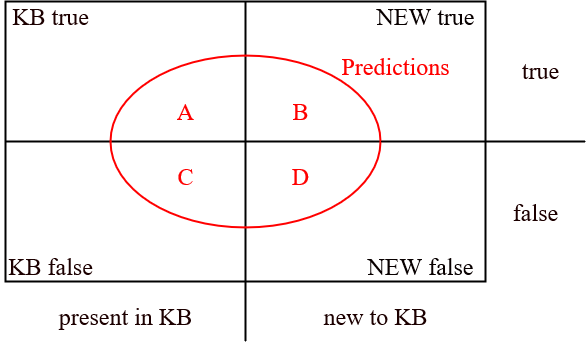
\includegraphics[width=10cm]{figures/kb_venn.png}
    \caption{KG prediction under incompleteness.}
    \label{KB_predictions}
\end{figure}

The OWA has a central problem regarding machine learning; it fails to provide counterexamples. Because missing facts are assumed to be neither true nor false, there are no false facts to give as examples when mining rules or training an embedding model. We used figure \ref{KB_predictions}, similar to the one used in the paper introducing AMIE \cite{amie}, to aid the explanation of solutions to this problem. The figure represents all possible triples given the relation $r$ and entities in a \gls{kg}. These triples can be split into four types:
\begin{enumerate}
    \item \gls{kg} true: True facts in the \gls{kg}
    \item NEW true: True facts not in the \gls{kg}
    \item \gls{kg} false: False facts \textit{known to} the \gls{kg}
    \item NEW false: False \textit{unknown to} the \gls{kg}
\end{enumerate}
When considering false facts we use the words ``\textit{known}" and ``\textit{unknown}" as a \gls{kg} generally does not contain false triples. We consider a given rule $B \Rightarrow r(x, y)$, where $B$ denotes the body of the rule and $r(x, y)$ the consequent. In figure \ref{KB_predictions} the red circle denotes predictions made by this rule. These predictions can be true and in the \gls{kg} (A), true and outside the \gls{kg} (B), false and known to be false (C) or false and unknown to be false (D). 

In the context of the predictions of the rule, we want to maximize B over D. Under the OWA, however, there are no false facts, so we do not know what B and D are. The authors of AMIE therefore introduced a new paradigm called the \textit{partial completeness assumption} (PCA) \cite{amie}. It assumes that if $r(x, y) \in KG true$ for some entities $x$, $y$, then
\[\forall y' : r(x, y') \in KGtrue \cup NEWtrue \Rightarrow r(x, y') \in KGtrue,\]
where $x$ is the \textit{head} of the triple (the first variable in the binary predicate) and $y$ is the \textit{tail} of the rule (the second varaible in the binary predicate).
This assumption says that if the \gls{kg} already has $r$-related information about the entity $x$,  then it contains \textit{all} $r$-related information about $x$. For example if a \gls{kg} only contains \texttt{(Ann, has\_sibling, Bob)} and no other sibling entries with Ann as the head, then by the PCA Bob is Ann's only sibling. All other facts claiming that Ann has other siblings will therefore be negative examples. If we then however ask what \textit{friends} Ann has in a knowledge base without information about Ann's friends, then one cannot conclude that Ann is friendless. PCA is a more particular version of the broad \textit{partial-closed world assumption} (PCWA), where the \gls{kg} generally is treated under the OWA, but parts of it that are considered complete are treated under the CWA \cite{motro1989integrity}. The PCA is more well-defined in the sense that it specifically states what parts of the \gls{kg} should be treated under closed-world semantics.

\section{Knowledge Graph Embeddings}
\label{KG_embeddings}
Let $\mathcal{K}$ be a \gls{kg} with triples of the form $(h, r, t)$ with $r\in \mathbb{P}$ and $h, t \in \mathbb{E}$, where $\mathbb{P}$ and $\mathbb{E}$ are respectively the set of all relations and the set of all entities entities in $\mathcal{K}$. Entities and relations are embedded in a vector space. To simplify the explanation we let the dimension of both entities and relations in the embedding space to be $d$.
Given $\mathcal{K}$ and $d$, a \gls{kge} seeks to represent all entities and relations in the continuous vector space of $d$ dimensions. These representations are meant to capture the semantic information in the graph. An embedding that manages this can then be used to evaluate the probability of new triples being true in the context of the \gls{kg} and identify false information in $\mathcal{K}$.%, two tasks respectively called \textit{link prediction} and \textit{triple classification}.

\begin{figure}[htp]
    \centering
    \includesvg[inkscapelatex=false,width=1\textwidth,keepaspectratio]{figures/KG_embeddings/KG_embedding_diag.svg}
    \caption[KGE process.]{\gls{kge} process. The embedding of a \gls{kg} can be used for machine learning tasks. Figure is based on work by Edoardo Ramalli \cite{wiki_KG_embedding}.}
    \label{KG_embdding_diag}
\end{figure}

The procedure for training \gls{kge} models is similar to any other statistical-based machine learning. The values of the embeddings are usually initialized as random values. These embeddings are continuously optimized through a training loop, which stops once the stop condition is met. A stop condition could be that a number of iterations have been completed, or when the model starts overfitting on the training set. For each triple in the training set, $\eta$ negative counterexamples are generated by triple corruption. This is done by swapping out either the head $h$ or tail $t$ (not both) with some other $h', t' \in \mathbb{E}$ \cite{TransE}. Both the original triple and the corrupted triples are added to the training batch. A \textit{scoring function} is used to measure the ``goodness" or plausibility of a triple. The model should give a good score to triples from the \gls{kg}, and a bad score to the corrupted triples. By updating the embedding to optimize the scoring function the model should at the end of training have meaningful embeddings that can accurately evaluate unseen triples. In the training process this is done by minimizing the model's \textit{loss function}.

\subsection{Loss functions}
A loss function is a function that assigns a ``cost" to an event in the form of a real number. The loss function is minimized with some optimization algorithm, such as stochastic gradient descent. If the reader is curious, this algorithm is well-described in the Deep Learning book by Goodfellow et al. \cite[p. 149]{goodfellow}. In the context of \gls{kge} models the loss function is used to update the embeddings \cite{dai2020survey}. There are many different types of loss functions, such as ranking losses \cite{TransE}, binary logistic regression \cite{complEx} and multiclass log loss \cite{kadlec2017knowledge}. We will briefly present the versions of ranking loss and multiclass log loss that were used in our experiments.

\subsubsection{Pairwise, margin-based ranking loss}
\textit{Learning to rank} is a machine learning task where a model is trained to rank a set of data points. In the \textit{pairwise} approach the problem is approximated to a binary classification problem, so the task becomes to determine which data point out of a pair is the better datapoint. The classifier takes as input two datapoints, one of higher rank $x_{+}$ and one of lower rank $x_{-}$, and has as goal to minimize the loss function which penalizes cases where $x_{-}$ is given a higher rank. So the goal is to create a ``gap" between positive and negative datapoints in the model's inner representation of the training data. In margin-based ranking loss a minimum value is set for this distance, so that once that distance is achieved the model no longer needs to make updates regarding the pair of datapoints with adequate distance, thereby allowing training to be spent on learning other more harder differences.  The authors of TransE use this pairwise, margin-based ranking approach as their loss function \cite{TransE}. Given a set of training triples $\mathcal{S}$, a scoring function $f$ and a margin $\gamma > 0$, the pairwise, margin-based ranking loss is defined as:

\[\mathcal{L}=\sum_{(h, r, t) \in \mathcal{S}}\sum_{(h', r, t') \in \mathcal{S'}}[\gamma + f(h, r, t) - f(h', r, t')]\]

where $\mathcal{S'}$ is the set of corrupted triples. This loss function favours low scores for corrupted triples and a high scores for non-corrupted triples. The aim is not to give negative triples a score below a certain value nor positive triples a score above a certain value, rather the goal is to create distance between them. This loss function can be used across many \gls{kge} models, as it is the \textit{scoring function} that differs across models. The scoring functions for TransE, DistMult and ComplEx will be presented in Section \ref{KG_embeddings_section}.


\subsubsection{Negative log-likelihood loss}
This loss function was used in the paper introducing ComplEx \cite{complEx}. Simply put, the function uses likelihood minimization to push the model toward the embedding that minimises the likelihood of loss. It is the \textit{opposite} of maximum likelihood estimation, where one wants to maximise the likelihood of some data points given a set of parameters, hence the name \textit{negative} log-likelihood.
Since the likelihood of facts in a \gls{kg} are independent, the likelihood of a set of triples is the same as the product of the likelihoods of each individual triple. With many of data points, multiplying many small probabilities with each other quickly leads to unmanageable small numbers. This causes \textit{underflow}, where a number is too small for a computer to be capable of storing it. To solve this problem, we take the log of the likelihoods so that products become sums. As log functions monotonically increase, the relative likelihood is maintained. For example if $f(h,r,t) \geq f(h', r, t')$ then $log(f(h,r,t)) \geq log(f(h', r, t'))$, so the $\geq$ is maintained. Since the goal is to create a distance between positive and negative triples, only the relative difference between them needs to be maintained. Thus the negative log-likelihood loss is:

\[\mathcal{L}=\sum_{(h, r, t) \in \mathcal{S} \cup \mathcal{S'}}log(1+exp(-y \, f(h, r, t)))\]

where $y\in [1, -1]$ is the truth value of the triple (true or false).


%This goes pretty in depth: %https://ieeexplore.ieee.org/stamp/stamp.jsp?tp=&arnumber=9416312

    
\subsection{Performance indicators}
\label{Performance_indicators}
Three different performance indicators are commonly used to evaluate the embedding quality of a model. While \gls{kge} models assign scores to triples, these scores are relative and cannot be used to give an absolute estimate of how well a model evaluates a triple. Instead, the scores are compared with those assigned to other triples so that the \textit{rank} of a triple can be used as an approximation of absolute measurement. A small rank number indicates a good rank, while a high rank value indicates a bad rank. This can be somewhat confusing, so the reader is encouraged to take care when distinguishing between rank ``number" and high/low rank, where a \textit{low} rank number indicates a \textit{high} rank and vice versa.

%Note that being ranked first (rank number 1) is best, and so when a fact is described as having a ``high rank" then the rank number itself is low. Similarly, if a triple has a low rank, the rank number assigned to it is high.

As the performance indicators are simple to calculate, they are suitable for measuring performance on a large scale. With $\mathcal{T}$ as the set of ranked triples and $\mathcal{S}$ as the set of true triples, we can define three performance indexes, as explained below.

\subsubsection{Hits@K}
\label{Hits@k}
Hits@K is the probability of finding the correct triple in the top K ranked triples. Usually $k=10$ or lower. This metric measures the model's ability to rank positive triples higher than corrupted ones.
\[\text{Hits@K}=\frac{|\{t\in \mathcal{T} : t_{rank}<k, t \in \mathcal{S}\}|}{|\mathcal{T}|}\]
The larger the value, the better the performance of the model.

\subsubsection{Mean rank}
Mean rank (MR) is the average rank of all the ranks assigned to the triples in the test set. A small value indicates a good model, because that means that more triples from the knowledge graph have been given higher ranks and accordingly, their rank numbers are smaller.
\[MR=\frac{1}{|\mathcal{T}|}\sum_{t\in\mathcal{T}}t_{rank}\]
MR has an advantage over Hits@K in being more sensitive to slight changes in the  model, because if the changes do not affect the top $k$ ranked triples then the Hits@K score remains unchanged.

\subsubsection{Mean reciprocal rank}
Mean reciprocal rank (MRR) is a measurement for the number of triples correctly ranked. If the triple with the best rank is a positive triple, then 1 is added. If the triple with the second best rank is positive, then $\frac{1}{2}$ is added, etc. If a ranked triple is negative nothing is deducted, the fraction simply is not added to the MRR.
\[MRR=\frac{1}{|\mathcal{T}|}\sum_{t\in\mathcal{T}}t_{rank} : t\in \mathcal{S}\]
The larger the value, the better the model.
    
\subsection{KG embedding model architectures}
\label{KG_embeddings_section}
\gls{kge} models differ mainly in three aspects: (1) how entities and relations are represented, (2) the scoring function, and (3) how the embedding is optimized. The difficulty with embedding \glspl{kg} is that there are many different entities and relationships, so the embedding model needs to be generic enough to capture all the different entities and relationships at the same time. We now consider the three models used in this thesis.

\subsubsection{TransE}
\label{TransE_peaked_in_2013}
In 2013, Mikolov et al. proposed a technique for natural language processing called \textit{word2vec} \cite{mikolov2013distributed,mikolov2013efficient}, which used a word-embedding algorithm that managed to capture some the of semantics in words. Words were represented as vectors, and the authors found that the embeddings had interesting qualities, such as
\[\overrightarrow{King} - \overrightarrow{Queen} \approx \overrightarrow{Man} -\overrightarrow{Woman}\]
where the words with an overhead arrow denote \textit{word2vec}'s vector embedding of the word. Inspired by this, Bordes et al. applied the idea to embedding entities and relations in \glspl{kg}, and proposed the embedding model TransE \cite{TransE}. A main motivation behind this approach was that ``\textit{hierarchical relationships are extremely common in KBs and translations are the natural transformations for representing them.}" \cite{TransE}. This approach learns entity embeddings and treats relations as translations in the entity embedding space.  For a true triple this means that the tail entity should be very close to the head entity plus the relation translation in the embedding space. 

\begin{figure}[htp]
    \centering
    \includesvg[inkscapelatex=false,width=0.4\textwidth,keepaspectratio]{figures/KG_embeddings/IKEA_TransE.svg}
    \caption[TransE embedding.]{Visualization of entity and relation embedding for TransE.}
    \label{IKEA_TransE}
\end{figure}

If $\text{\textbf{(h, r, t)}}$ denote an embedding of a head, relation and tail, then $\textbf{h} + \textbf{r} \approx \textbf{t}$. The score function $f_{TransE}$ is thus defined as the distance between $\textbf{h} + \textbf{r}$ and $\textbf{t}$, using $l_1$ or $l_2$ to calculate distance:
\[f_{TransE}(h, r, t) = ||\textbf{h} + \textbf{r} - \textbf{t}||_{l_1/l_2}\]

Let $d$ denote the dimension of the embedding space. Per entity one vector $\textbf{e}\in \mathbb{R}^d$ needs to be learned and per relationship one translation vector $\textbf{d}_r\in \mathbb{R}^d$ needs to be learned. Let $n_e$ and $n_r$ be the number of unique entities and relations respectively. The number of parameters needed to be learned for TransE is thus $\mathcal{O}(n_e d + n_r d)$.


TransE does have some limitations. For example, it is not capable of properly embedding complex relations, meaning 1-N, N-1, or N-N relations \cite{transH, transR}. Imagine a complex relation such that $\forall i \in \{1,2, ..., n\}$, $(h, r, t_i )\in \mathcal{S}$, where $\mathcal{S}$ is the set of correct triples. Following the TransE approach, $\textbf{h}+\textbf{r}\approx \textbf{t}_i$, therefore $\textbf{t}_1 \approx \textbf{t}_2 \approx ... \approx \textbf{t}_i$, even though the tail entities are not necessarily semantically similar. Taking an example depicted in figure \ref{IKEA_TransE}, the store IKEA sells both furniture and food, causing TransE to give the semantically dissimilar concepts a similar entity embedding. 

For a symmetric relation $r_{sym}$, TransE will assign high scores to both $(h, r_{sym}, t)$ and $(t, r_{sym}, h)$. This results in the embedding for $r_{sym}$ to be pushed toward zero in addition to the embedding of the entities $h$ and $t$ toward each other \cite{wang2018evaluating}. When $r_{sym} \approx 0$, then the relation is treated as if it were reflexive. This is problematic when embedding symmetric relations, especially those that additionally are \textit{not} reflexive. Other translation-based models, such as TransH \cite{transH}, TranR \cite{transR} and TransD \cite{transD}, have later been proposed to alleviate some of the limitations of TransE.

\subsubsection{DistMult}
DistMult is based on the tensor factorization-based model RESCAL \cite{RESCAL}. A tensor is a multidimensional array that represents the relationships between muliple sets of objects. The dimension of the array is the number of types of objects in the combinations. In the context of triples there is the head entity, the relation and the tail entity, so three sets of object types. In such models triples in a \gls{kg} are therefore transformed into a 3D binary tensor $\mathcal{X}$. We want the embeddings of the entities and relations to be such that one can mathematically combine them to obtain the tensor representing the \gls{kg}. As seen in \cref{tensor_model_fig}, in the \gls{kg} tensor each relation is represented by an $n \times n$ matrix, where $n$ is the number of unique entities. The number of relations is denoted by $m$, so $\mathcal{X}\in \mathbb{R}^{n \times n \times m}$. An element $X_{ijk} = 1$ if there is a triple $(e_i, r_j, e_k)$ in the graph, and $X_{ijk} = 0$ otherwise.

\begin{figure}[htp]
    \centering
    \includesvg[inkscapelatex=false,width=0.4\textwidth,keepaspectratio]{figures/KG_embeddings/DistMult_matrices.svg}
    \caption[A tensor model of a knowledge graph.]{A tensor model of a knowledge graph, inspired by the figure by Dai et al. \cite{dai2020survey}.}
    \label{tensor_model_fig}
\end{figure}

RESCAL uses rank-$d$ factorization to obtain the latent semantics \cite{RESCAL}. The \textit{rank} of a matrix corresponds to the number of linearly independent columns in it. Given a matrix $\mathcal{Y} \in \mathbb{R}^{n\times m}$ of rank $o$, the rank fatorization of $\mathcal{Y}$ is of the form $\mathcal{Y}=FG$ where $F\in \mathbb{R}^{m\times r}$ and $G\in \mathbb{R}^{r\times o}$. For $\mathcal{X}$ the rank factorization is applied so that tensor is ``split" into slices, where each slice corresponds to the semantic embedding of a relation. Rank $d$ is used, because the relations are embedding in $d \times d$-dimensional space. Formally we can define the $p$th slice in the \gls{kg} tensor as:
\begin{center}
 $\mathcal{X}_p \approx AR_p A^T$, for $p = 1,2,...,m$
\end{center}
where $A\in \mathbb{R}^{n\times d}$ is the matrix representing all entities and $R_k\in \mathbb{R}^{d\times d}$ is a matrix representing the $p$th relation.
So the scoring function used in RESCAL is
\[f_ {\text{RESCAL}}(h, r, t) =\textbf{h}^{\top}\textbf{M}_r\textbf{t}\]
where $\textbf{h, t}\in \mathbb{R}^{d}$ are the embedding vectors of entities and $\textbf{M}_r \in \mathbb{R}^{d\times d}$ is the semantic embedding of the relation.
This method requires thus $\mathcal{O}(n_ed + n_r d^r)$ parameters. In order to lower this complexity, DistMult restricts $\textbf{M}_r$ to be a diagonal matrix, meaning that all entries apart from those in the diagonal of the matrix are zero. After $\textbf{M}_r = \text{diag}(\textbf{r}), \textbf{r}\in\mathbb{R}^d$. The scoring function is transformed to
\[f_ {\text{DistMult}}(h, r, t) =\textbf{h}^{\top}\text{diag}(\textbf{r})\textbf{t}\]
Now only $d$ parameters need to be learned per relationship, and the number of parameters to be learned for DistMult is $\mathcal{O}(n_ed + n_r d)$. The space required is also $\mathcal{O}(n_ed + n_r d)$.

A main problem with this approach is that $f_ {\text{DistMult}}(h, r, t) = f_ {\text{DistMult}}(t, r, h)$, so DistMult cannot embed the asymmetry of a relation. This issue is addressed by later models, such as ComplEx \cite{complEx} and SimplE \cite{SimplE}.


\subsubsection{ComplEx}
ComplEx extends DistMult with complex-valued embeddings, thereby allowing it to distinguish between symmetric and asymmetric facts \cite{complEx}. This was achieved without increasing parameter or memory complexity. The imaginary and real part of the embeddings play the role of representing the ``direction" of the relation and thus asymmetric qualities can be expressed in the embedding. The scoring function for ComplEx is quite similar to that of DistMult:
\[f_ {\text{ComplEx}}(h, r, t) =\textbf{Re}(\textbf{h}^{\top}\text{diag}(\textbf{r})\overline{\textbf{t}})\]
where $\overline{\textbf{t}}$ represents the complex conjugate of \textbf{t} and \textbf{Re} means we are taking the real values of the score. With such a scoring function, triples with asymmetric relations are able to obtain different scores depending on the ordering of entities.
    

\section{Rule-based machine learning}
Rule-based machine learning has as a goal to create rules that make new true predictions going beyond the data on which the rule was applied to \cite{weiss1995rule}. Other areas of statistical machine learning often focus on training a single model that can be applied to make a broad range of predictions. Conceptually, the end result of rule-based machine learning is similar to a rule-based system.  Rule-based systems are often hand-crafted and require a knowledge expert to be curated, while rule-based machine learning requires no knowledge expert and rules are automatically created by the learning algorithm.

Classically, a rule is comprised of a condition and consequent, or a so-called "if-then" statement. \begin{center} \textbf{IF} \textit{`the condition is met'} \textbf{THEN} \textit{`the consequent holds'} \end{center}
The condition of the rule specifies attributes in the data on which the rule will be applied. If these attributes are present in this data, the condition is met. Once this happens, the attributes in the consequent should necessarily also be met. We define an \textit{atom} to be a triple in which the head and/or tail are variables. A \textit{Horn rule} is a rule where the consequent of a rule is a single atom, while the body is a set of atoms. We denote a Horn rule by $B \Rightarrow r(x, y)$ where $B$ is the antecedent and $r(x, y)$ the consequent. Two examples of such rules are \ref{example_rule_1} and \ref{example_rule_2}, where the first is satisfied by the \gls{kg} in Example \ref{mini_KG_rules} below, while the latter is not.
\begin{equation}
has\_sibling(x, y) \Rightarrow has\_sibling(y,x)
\label{example_rule_1}
\end{equation}
\begin{equation}
    has\_sibling(x, y), has\_parent(y,z) \Rightarrow has\_parent(x,z)
    \label{example_rule_2}
\end{equation}


\begin{example}[A simple KG.]
\begin{lstlisting}[]
(Ann, has_parent, Carol)
(Carol, has_child, Ann)
(Carol, has_child, Bob)
(Ann, has_sibling, Bob)
(Bob, has_sibling, Ann)
\end{lstlisting}
\label{mini_KG_rules}
\end{example}


Consider the two rules and the example \gls{kg} with numbered triples given above. Under this knowledge base the antecedent of the first rule is satisfied by both triple 4 and 5 listed in the example. The resulting consequent of rule \ref{example_rule_1} is also present in the knowledge base. So the predicate $has\_sibling$ is reflexive in this knowledge base. The antecedent of the second rule is satisfied by triples 1 and 5 in the knowledge base, but the resulting consequent would then be $has\_parent(Bob, Carol)$. Since \texttt{(BoB, has\_parent, Carol)} is not present in the knowledge base, rule \ref{example_rule_2} does not hold. If we know that this rule is reliable, we could for example extend the incomplete knowledge base with this triple.

Within rule-based machine learning there are many different approaches, including learning classifier systems \cite{sigaud2007learning} and association rule mining \cite{agrawal1993mining}, the latter of which is the approach used in this thesis. Both approaches aim to create a set of rules to act as a model for a set of data. The association rule mining approach will now be explained further.


\subsection{Association rule mining}
Association rules \cite{agrawal1993mining} are types of ``if-then" statements that describe frequent associations between items in a dataset containing \textit{transactions}. A transaction can be thought of as a set of related items. Association rule mining was originally proposed as a new method for finding relationships between sales items in stores. The idea of mining association rules over transactions has successfully been applied to many other scenarios, such as within health informatics and reccomender systems \cite{altaf2017applications, lin2002efficient}. In the context of convenience store sales, each transaction can be thought of as a set of items that a customer has purchased. The rules are of the form $\{Sugar, Flour, Eggs\} \Rightarrow Butter$, meaning that a person who bought sugar, flour and eggs is likely to also purchase butter. The antecedent is some set of items in the dataset, while the consequent is an item often found in combination with the antecedent in the dataset.  So sugar, flour and eggs can be thought of as ``associated with" butter. These original association rules are also not Horn rules over binary predicates as in AMIE3, but it is cited as a main inspiration for the AMIE3 algorithm used for experiments in this thesis. AMIE3 also limits rules to be in Horn form, meaning that the consequent can contain at most one predicate.

\subsection{Significance and quality measurement}
\label{significance_and_quality}
The goal is to find formal rules that make true predictions that go beyond the explicit information in the knowledge base. If we look back at \cref{KB_predictions} this means we want to maximise B and minimise D. For this we need to know what those areas are, and this is where the problem of missing negative examples from \cref{Integrity_of_KGs} occurs as the area \textbf{KB false} is empty. While it is hard to define \textit{quality} when evaluating rules, there are some indicators that can be used. We now consider different measures addressing this problem.

\subsubsection{Support}
The \textit{support} of a rule is the quantity of correct predictions. If we recall figure \cref{KB_predictions} with \gls{kg} prediction under incompleteness, the support of a rule $B \Rightarrow r(x,y)$ is area A. What counts as an instance of a correct prediction can vary. The authors of AMIE point out that if one chooses the number of instantiations of the rule, then the measure becomes non-monotonic \cite{amie3}. They give an example with the rule:
\[married\_to(x, y) \Rightarrow married\_to(y, x)\]
where if $has\_gender(x, male)$ is added to the body, then the number of instantiations in the \gls{kg} can only decrease because there are stricter requirements for what can be in the body of the rule. If on the other hand $has\_friend(x, z)$ is added to the body then the number of instantiations may increase,because for every $x$ there can be many $z$ possibly resulting in many more instantiations of the rule. In order to preserve monoticity and only a single measure of support for each rule, the authors of AMIE define support of a rule $R$ to be the number of true predictions $p$ in the \gls{kg} $\mathcal{K}$ that the rule makes:
\[support(R) :=  | \{p : (\mathcal{K} \wedge R \models p)\wedge p \in \mathcal{K} \}|\]
Now the support of a rule decreases monotonically if more atoms are added to the body, and two equivalent rules cannot have different values for support.

\subsubsection{Head coverage}
Support is not an absolute measurement, rather a relative measurement. It requires the complete size of the \gls{kg} for the values to have meaning. This is countered with a proportional version of support called \emph{head coverage}. Given a rule $B \Rightarrow r(x,y)$, the head coverage is the ratio of instantiations of the head of the rule $r(x, y)$ that are predicted by the rule:
\[hc(B \Rightarrow r(x,y)) = \frac{support(B \Rightarrow r(x,y))}{|\{(x, y) : r(x, y) \in \mathcal{K}}|\]
Head coverage is fully correlated with support, and hence is also monotonic. We now have an absolute measurement of significance, but this is not a measure of quality of a rule, only relevance. For this we need confidence measures.


\subsubsection{Standard Confidence} Confidence is the proportion of a rule's true predictions out of all its predictions. In order to determine if a new fact is true or false, one must make assumptions about the facts missing from the \gls{kg}. The \textit{standard confidence} adopts the CWA and labels all facts not already present in the \gls{kg} as false. Thus, the standard confidence of a rule $R$ in a \gls{kg} $\mathcal{K}$ is the ratio of its predictions that are in the KG:
\[conf(R) := \frac{support(R)}{support(R) + | \{p : (\mathcal{K} \wedge R \models p)\wedge p \not\in \mathcal{K} \}|}\]

If we take the \gls{kg} from Example \ref{mini_KG_rules} and the rule $has\_child(y, x) \Rightarrow has\_parent(x, y)$, then the rule implies two datapoints: \texttt{(Ann, has\_parent, Carol)} and \texttt{(Bob, has\_parent, Carol)}. The first triple is in the \gls{kg}, while the second is not, therefore the rule has predicted one correct and one incorrect triple, thus the standard confidence is 0.5.


If one wants to mine rules that only describe the data at hand, and has a relatively complete \gls{kg}, then this is a good measure of confidence. If the aim on the other hand is to mine rules that predict new facts then standard confidence is not a good measurement as it penalizes rules that make predictions outside of the current knowledge.


\subsubsection{PCA Confidence}
This measurement for confidence differs from standard confidence in its definition of what is a false prediction. Under standard confidence any triple outside the \gls{kg} is a false prediction, while this confidence metric adopts PCA, introduced in section \ref{Integrity_of_KGs}. The definition of a false prediction is thus more conservative, so not all triples outside the \gls{kg} are considered false. The PCA confidence of the rule $R$ is the fraction of its predictions that are not labeled as false by the PCA \cite{amie}:
\[pca-conf(B\Rightarrow r(x, y)) := \frac{support(B\Rightarrow r(x, y))}{|\{(x, y):\exists y' : B \wedge r(x, y')\}|}\]

Again, given the \gls{kg} from Example \ref{mini_KG_rules} and the rule $has\_child(x, y) \Rightarrow has\_parent(y, x)$, the rule implies two datapoints: \texttt{(Ann, has\_parent, Carol)} and \texttt{(Bob, has\_parent, Carol)}. The first is in the \gls{kg}, therefore correct, while the latter is outside the \gls{kg}. As there are no \texttt{has\_parent} triples with \texttt{Bob} as the subject in the \gls{kg}, we cannot under the PCA assume that \texttt{(Bob, has\_parent, Carol)} is a false triple. Hence, the PCA confidence of the rule is 1.0, in contrast to the standard confidence of 0.5.

This is the standard PCA confidence measure, but it could of course also be calculated on the head entity of the consequent instead of the tail, ie.: 
\[pca-conf_h(B\Rightarrow r(x, y)) := \frac{support(B\Rightarrow r(x, y))}{|\{(x, y):\exists x' : B \wedge r(x', y)\}|}\]

Note that the PCA confidence calculated on the \textit{tail} of the consequent is the metric used throughout this thesis to indicate the quality of rules.

\subsubsection{GPRO and GRANK confidence}
The work of Ebisu et al. \cite{gpro} showed that PCA confidence may underestimate the likelihood of a predicted triple due to non-unique mappings of variables in rules. Consider for example the rule $has\_parent(x, z) \wedge has\_child(z, y) \Rightarrow has\_sibling(x, y)$, and the \gls{kg} from Example \ref{mini_KG_rules}. By mapping both $x$ and $y$ to the entity \texttt{Ann}, body of this rule can be instantiated with the triples \texttt{Ann, has\_parent, Carol} and \texttt{(Carol, has\_child, Ann)}, resulting in the incorrect fact that Ann is her own sibling. The refinement of PCA confidence, called \textit{graph pattern probability model} (GRPO) confidence, excludes instances such as these that do not map variables to unique entities when computing confidence. As with PCA confidence, GPRO confidence can be calculated on both the head and tail of the consequent.

Ebisu et al. also proposed a refinement of GPRO confidence, called GRANK confidence \cite{gpro}, which takes into account the number of instantiations of the body of the rule for a given instantiation of the head atom. This metric is more sensitive to the number of facts per relation.


\subsection{AMIE, AMIE+ and AMIE3}
\label{the_amies}
The experiment of this thesis required a rule miner which could mine meaningful rules and maintain an acceptable time to complete. This component of the experiment would be treated as a black box that only took a \gls{kg} as input and produced a set of rules as output. The AMIE-algorithms do exactly this, and require no hyperparameter optimization, training, nor additional input.

AMIE is a rule mining system introduced in 2013 by Galárraga et al. \cite{amie}, which was improved upon in 2015 with the release of AMIE+ \cite{amie_plus} and in 2020 with AMIE3 \cite{amie3}. This section will summarise the original rule mining algorithm, present the improvements made with AMIE+ and AMIE3, and finally justify the eventual choice of AMIE3.

\subsubsection{The AMIE rule mining algorithm}
The algorithm employs a type of breadth first search when exploring the search space for possible rules. It starts with the empty rule, which it and extends it. It is extended in a way that if this breadth-first extension continues, the entire search space can be generated. This is of course not desired, and so AMIE employs a number of methods to limit the search for rules. One can think of this as methods of pruning the breadth first search tree. We first explain how rules are extended, and then how the search space is pruned.

A rule is treated as a sequence of atoms, where the first atom is the head and the rest make up the body. It is considered \textit{closed}, if every variable is shared by at least two predicates. These rules can also be thought of as \textit{closed-path} rules, as the sequence of relations in the body of the rule form a path from the subject argument to the object argument of the head atom in the rule. The rule $has\_child(y, x) \Rightarrow has\_parent(x, y)$ is closed. If we were to add an atom to the body with a fresh (new and unused) variable, a resulting rule $has\_sibling(z, x) \wedge has\_child(y, x) \Rightarrow has\_parent(x, y)$, would be open. The algorithm only outputs closed rules, which ensures that rules do not contain unrelated atoms or variables. When traversing the search space, AMIE extends rules by adding one of three different atom types:
\begin{enumerate}
    \item \textit{Dangling atom}: An atom with a fresh variable and a shared variable is added. A shared variable is a variable that occurs in some other atom of the rule.
    \item \textit{Instantiated atom}: An atom with an entity and an argument (variable or entity) shared with the rule.
    \item \textit{Closing atom}: An atom with both arguments shared with the rule.
\end{enumerate}

By only adding atoms to rules the extension is monotonic in the sense that atoms added by one operation cannot be modified by a later operation. In the algorithm new rules are added to a queue. If however a generated rule is a duplicate of one already in the queue, it is not enqueued. Because the length of the rules dequeued increases monotonically, one can be sure that any potential duplicates still are in the queue -- when a rule with $n$ atoms is dequeued, no rule with $n+1$ atoms has ever been dequeued. Since rules that are equal have the same head coverage and PCA confidence, this limits the search space considerably when checking for duplicates before enqueuing a new rule.

The head coverage of possible rules must be at least 0.01, meaning rules that correctly predict less than 1\% of the head relations are deemed insignificant. As mentioned in section \ref{significance_and_quality} \textit{head coverage} decreases monotonically as atoms are added to a rule. This allows the algorithm to safely discard and not expand upon rules that score below the head coverage threshold. With the default setting a rule also needs support $\geq$ 100. %The monoticity of head coverage also allows the algorithm to stop expanding upon rules for which a smaller version has larger confidence. The PCA confidence and head coverage of the smaller rule must be higher than that of the larger.

For more details about the implementation details of AMIE please refer to the original paper, \textit{AMIE: association rule mining under incomplete evidence in ontological knowledge bases} \cite{amie_plus}. Note that the authors of AMIE present results with rules mined \textit{without} constants, unless it is explicitly stated. This is also the case for the AMIE+ and AMIE3 publications. The AMIE-algorithms are capable of mining rules with instantiated atoms, but at the expense of increased time required to run.

\subsubsection{AMIE+ and AMIE3}
While the original AMIE algorithm had some intelligent methods for limiting the search space, it spent 3.62min on a server with 48GB RAM and 8 CPUs \cite{amie} when mining rules with two atoms and no constants from YAGO2, which has around 1 million facts \cite{yago2}. In recent years knowledge bases have only increased in size (YAGO4 has 2 billion facts \cite{yago4}), and so the improvements made in AMIE+ and AMIE3 address this need for improved performance. AMIE+ includes new pruning techniques, such as the fact that rules with 100\% confidence cannot be improved upon, hence do not need to be expanded. Computing the PCA confidence of rules is a quite expensive part of the algorithm, so AMIE+ introduces a method for approximating the confidence score. This approximation has a 4\% error rate, but shortens the runtime considerably. AMIE3 uses more sophisticated methods for calculating support and PCA confidence, and does not need to resort to approximations, while improving runtime. It also employs a technique called \textit{lazy evaluation}, which rests on the idea that if a rule is bad, there is no need to spend resources calculating exactly how bad it is. 

Depending on the intended application of the mined rules, different metrics are more appropriate than others. For example, standard confidence is more appropriate if one assumes that the information in the \gls{kg} is complete and one wants rules that model the data as closely as possible. If the intended use of the rules on the other hand is to predict new facts, then PCA, GPRO or GRANK confidence are more appropriate. In release of AMIE3 all these metrics are implemented, however their implementation of GPRO or GRANK confidence was still in the experimental stages, therefore PCA confidence was used in this thesis.


\subsubsection{The role of AMIE3 in experiments}
The rule miner required for the experiments in this master project had to have reasonable running time and have the ability to mine rules of acceptable quality. The PCA confidence measure, while not perfect, was deemed an adequate indication of quality, and therefore the AMIE-algorithms that employed this measure seemed appropriate for the task. The AMIE3 algorithm was of course the best of the three, and it performed well against other recent rule mining algorithms, such as Ontological Pathfinding \cite{op} and RudiK \cite{rudik}. Furthermore, the authors of AMIE3 had made their publication publicly available on GitHub with clear instructions on how to use it. For these reasons the AMIE3 algorithm was chosen as the rule miner for the experiments of the present project.








\iffalse 
\section{Web Ontology Language}
A widely used formal language for expressing ontologies is the \gls{owl}. In OWL "Daughters are female" could be formally expressed as:

\centerline{\textsf{SubClassOf(Daughter Female)}}
Information expressed in OWL can be used to draw new conclusions. For example if we know that an individual \emph{Amy} is a daughter, then we can makes the same conclusions as earlier about Amy being female. In OWL, the fact that Amy is in the class of females can be expressed as:

\centerline{\textsf{ClassAssertion(Female amy)}}
The task of reaching such conclusions is called reasoning and the type of conclusions that can be drawn is specified by the \gls{w3c}. It specifies the \emph{semantics} of OWL, but does not present algorithms for how to derive inferences in practice. Sound and complete reasoning in OWL is of high complexity \cite{Krotzsch2012}. Therefore, when the standard was updated to OWL 2 in 2009, it introduced restricted sublanguages to address this problem. These sublanguages restrict expressivity in order to simplify the reasoning task. One of these languages is OWL 2 QL, which is based on a \gls{dl} language called DL-Lite. OWL 2 QL is intended as a language to enable easier queries to databases. The ontology language we will use is DL-Lite$_{\mathcal{R}, horn}^{\exists}$, which is a member of the DL-Lite family.



\section{Description Logics}
\gls{dls} are a family of languages used in knowledge representation and reasoning. They are generally less expressive than \gls{fol}, but more expressive than \gls{pl}. The name \textit{description logic} represents two central aspects to this language group: \emph{description}, formal expression of knowledge, and  \emph{logic}, for it's logic-based semantics. DLs are used to represent domain knowledge in a well-structured and easily interpretable way. Domain knowledge is separated into two components in DL, a \emph{terminological} part, called a TBox, and an \emph{assertional} part, called an ABox. The TBox represents knowledge about the structure of the domain, while the ABox has knowledge about specific instances. For example the fact that \emph{cats are  mammals} would be a TBox statement, while \emph{Leo is a cat} would be an ABox statement, as here we are making an assertion about the individual Leo. The combination of a TBox and an ABox is called a \emph{knowledge base} (KB).
As the semantics of DLs are logic-based it is clear when a statement is \emph{entailed} by a KB. For instance the two examples given above entail that Leo is a mammal. More importantly, this reasoning task can be automated in a DL KB. Reasoning tasks are performed with respect to the entire KB, which gives this language great power, but also comes with a computational cost. Therefore an important area of research has been to find DLs that strike a balance between expressiveness and the computational complexity of reasoning.


The two main criteria for a reasoner is that it is decidable and tractable (always correctly completed in a time that is polynomial with respect to the size of the KB). The more operators one allows in a logic the more complicated the TBox becomes, and usually the complexity for reasoning in the language increases. See \href{http://www.cs.man.ac.uk/~ezolin/dl/}{\textbf{Complexity of reasoning in Description Logics}} for an interactive look at the complexity of different DLs \cite{zolin_2013}.

\section{The Resource Description Framework}

The Resource Description Framework (RDF) is a standard for representation and exchange of graph data introduced by \gls{w3c}. Semantic triples are the data types used in the RDF data model. A triple, as the name suggests, is a tuple of three elements. It has the form ( subject, predicate, object) and can therefore represent statements about semantic data, for example "Cats are mammals", or "Ann knows Bob". These RDF statements express relationships between two resources, these resources being the subject and the object, while the predicate encapsulates the nature of the relationship. The relationship is phrased in a directional way, and so set of RDF stamements can also be viewed as a directed graph. The graph represents these triple statements, where the predicate in the triple denotes the edge going from the subject to the object, both of which are vertices.

\begin{lstlisting}[caption={Example of RDF triple set written in informal pseudocode},label={RDF_triples_example}]
<Ann> <knows> <Bob>
<Ann> <is a> <person>
<Bob> <is a> <person>
<Ann> <owns> <Leo>
<Leo> <is a> <cat>
<cat> <is a> <mammal>
<Bob> <is scared of> <Leo>
\end{lstlisting}

\begin{figure}
\centering
    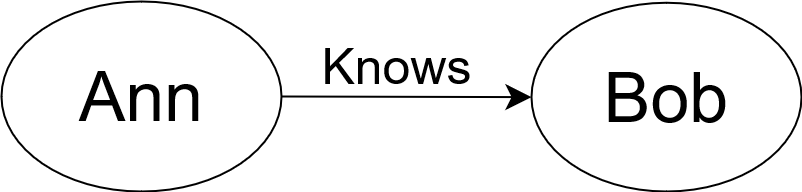
\includegraphics[scale=0.3]{figures/RDF_triple}
    \caption{TODO Informal graph of the example triples from \ref{RDF_triples_example}}
    
    \label{fig:RDF_figure}
\end{figure}

With this type of data organisation one can for example query for a list of all people who own cats in the dataset.

\subsection{Resource Description Framework Schema}
RDF provides the abstract model for how to organize the data and sets standards for how data points relate to eachother and real-world entities. The RDF Schema (RDFS), on the other hand, is a \emph{vocabulary} in RDF that explains how nodes of a graph relate.

\section{Semantic Triples in Description Logics}
Semantic triples are 
\fi
